\documentclass[12pt]{article}\usepackage[]{graphicx}\usepackage[]{color}
%% maxwidth is the original width if it is less than linewidth
%% otherwise use linewidth (to make sure the graphics do not exceed the margin)
\makeatletter
\def\maxwidth{ %
  \ifdim\Gin@nat@width>\linewidth
    \linewidth
  \else
    \Gin@nat@width
  \fi
}
\makeatother

\definecolor{fgcolor}{rgb}{0.345, 0.345, 0.345}
\newcommand{\hlnum}[1]{\textcolor[rgb]{0.686,0.059,0.569}{#1}}%
\newcommand{\hlstr}[1]{\textcolor[rgb]{0.192,0.494,0.8}{#1}}%
\newcommand{\hlcom}[1]{\textcolor[rgb]{0.678,0.584,0.686}{\textit{#1}}}%
\newcommand{\hlopt}[1]{\textcolor[rgb]{0,0,0}{#1}}%
\newcommand{\hlstd}[1]{\textcolor[rgb]{0.345,0.345,0.345}{#1}}%
\newcommand{\hlkwa}[1]{\textcolor[rgb]{0.161,0.373,0.58}{\textbf{#1}}}%
\newcommand{\hlkwb}[1]{\textcolor[rgb]{0.69,0.353,0.396}{#1}}%
\newcommand{\hlkwc}[1]{\textcolor[rgb]{0.333,0.667,0.333}{#1}}%
\newcommand{\hlkwd}[1]{\textcolor[rgb]{0.737,0.353,0.396}{\textbf{#1}}}%
\let\hlipl\hlkwb

\usepackage{framed}
\makeatletter
\newenvironment{kframe}{%
 \def\at@end@of@kframe{}%
 \ifinner\ifhmode%
  \def\at@end@of@kframe{\end{minipage}}%
  \begin{minipage}{\columnwidth}%
 \fi\fi%
 \def\FrameCommand##1{\hskip\@totalleftmargin \hskip-\fboxsep
 \colorbox{shadecolor}{##1}\hskip-\fboxsep
     % There is no \\@totalrightmargin, so:
     \hskip-\linewidth \hskip-\@totalleftmargin \hskip\columnwidth}%
 \MakeFramed {\advance\hsize-\width
   \@totalleftmargin\z@ \linewidth\hsize
   \@setminipage}}%
 {\par\unskip\endMakeFramed%
 \at@end@of@kframe}
\makeatother

\definecolor{shadecolor}{rgb}{.97, .97, .97}
\definecolor{messagecolor}{rgb}{0, 0, 0}
\definecolor{warningcolor}{rgb}{1, 0, 1}
\definecolor{errorcolor}{rgb}{1, 0, 0}
\newenvironment{knitrout}{}{} % an empty environment to be redefined in TeX

\usepackage{alltt}         % the type of document and font size (default 10pt)
\usepackage[margin=1.0in]{geometry}   % sets all margins to 1in, can be changed
\usepackage{moreverb}                 % for verbatimtabinput -- LaTeX environment
\usepackage{url}                      % for \url{} command
\usepackage{amssymb}                  % for many mathematical symbols
\usepackage[pdftex]{lscape}           % for landscaped tables
\usepackage{longtable}                % for tables that break over multiple pages
\usepackage[normalem]{ulem}
\useunder{\uline}{\ul}{}

\title{Energy Building Analysis}  % to specify title
\author{Alexander Kell}          % to specify author(s)
\IfFileExists{upquote.sty}{\usepackage{upquote}}{}
\begin{document}                      % document begins here

% If .nw file contains graphs: To specify that EPS/PDF graph files are to be 
% saved to 'graphics' sub-folder
%     NOTE: 'graphics' sub-folder must exist prior to Sweave step
%\SweaveOpts{prefix.string=graphics/plot}

% If .nw file contains graphs: to modify (shrink/enlarge} size of graphics 
% file inserted
%         NOTE: can be specified/modified before any graph chunk
\setkeys{Gin}{width=1.0\textwidth}

\maketitle              % makes the title
%\tableofcontents        % inserts TOC (section, sub-section, etc numbers and titles)
%\listoftables           % inserts LOT (numbers and captions)
%\listoffigures          % inserts LOF (numbers and captions)
%                        %     NOTE: graph chunk must be wrapped with \begin{figure}, 
%                        %  \end{figure}, and \caption{}
%%%%%%%%%%%%%%%%%%%%%%%%%%%%%%%%%%%%%%%%%%%%%%%%%%%%%%%%%%%%%%%%%%%%
% Where everything else goes


\section{Introduction}

Analysing different buildings based on their energy usage can bring us many benefits. We can understand what amounts of energy people use, how they use it, and why they use it. All this information can lead us to new insights. 
\\\\
Insights such as these enable us to target customers, and persuade them to change their usage habits, or inform us on the type of financial products users may require. \\

Having a thorough analysis on usage habbits can help us during the planning stage of electricity generation, especially when these are matched to weather conditions. \\

\section{Explanation of Data}

Firstly I downloaded data from the following website:\\
http://en.openei.org/datasets/dataset/commercial-and-residential-hourly-load-profiles-for-all-tmy3-locations-in-the-united-states.

This contains data from multiple buildings, recorded every hour for the entire year of 2004.

The data is made up of 15,000 CSV files. Each file contains an hourly breakdown of different usages of energy. Such as the overall amount of electricity used per hour, and overall amount of gas used per hour. There is also more specific data such as what was using the electricity and gas. \\

The specific data is broken down into usage of heating, cooling, interior lights, exterior lights, water heating, interior gas equipment, and interior electricity equipment.\\

A total of 8,760 samples are recorded per building. These correspond to each hour within a given year.\\

The data is made up of many different building types, which are displayed below. 

\begin{table}[]
\centering
\label{my-label}
\begin{tabular}{|l|}
\hline
\textbf{Type of Building} \\ \hline
Stand Alone Retail        \\ \hline
Mall                      \\ \hline
Secondary School          \\ \hline
Primary School            \\ \hline
Medium Office             \\ \hline
Large Office              \\ \hline
Small Hotel               \\ \hline
Apartment                 \\ \hline
Full Service Restaurant   \\ \hline
Quick Service Restaurant  \\ \hline
Hospital                  \\ \hline
Supermarket               \\ \hline
Warehouse                 \\ \hline
\end{tabular}
\caption{Types of buildings available in data}
\end{table}

\section{Analysis}
\subsection{Data Manipulation}





The first step was to import the data into a single data frame into R. The data imported was electricity usage of each building.




I began by converting the data into an R friendly format. Namely, by converting the time and date information into a format suitable for R.




Next information was extracted such as the day of the week, month, and hour. This enabled me to quickly plot the data and begin exploring the data.




\subsection{Early Stage Plotting}

I plotted all the electricity used over a year throug the use of boxplots. Each boxplots relates to a different month and enables us to see average changes in electricity over a year.

\begin{knitrout}
\definecolor{shadecolor}{rgb}{0.969, 0.969, 0.969}\color{fgcolor}
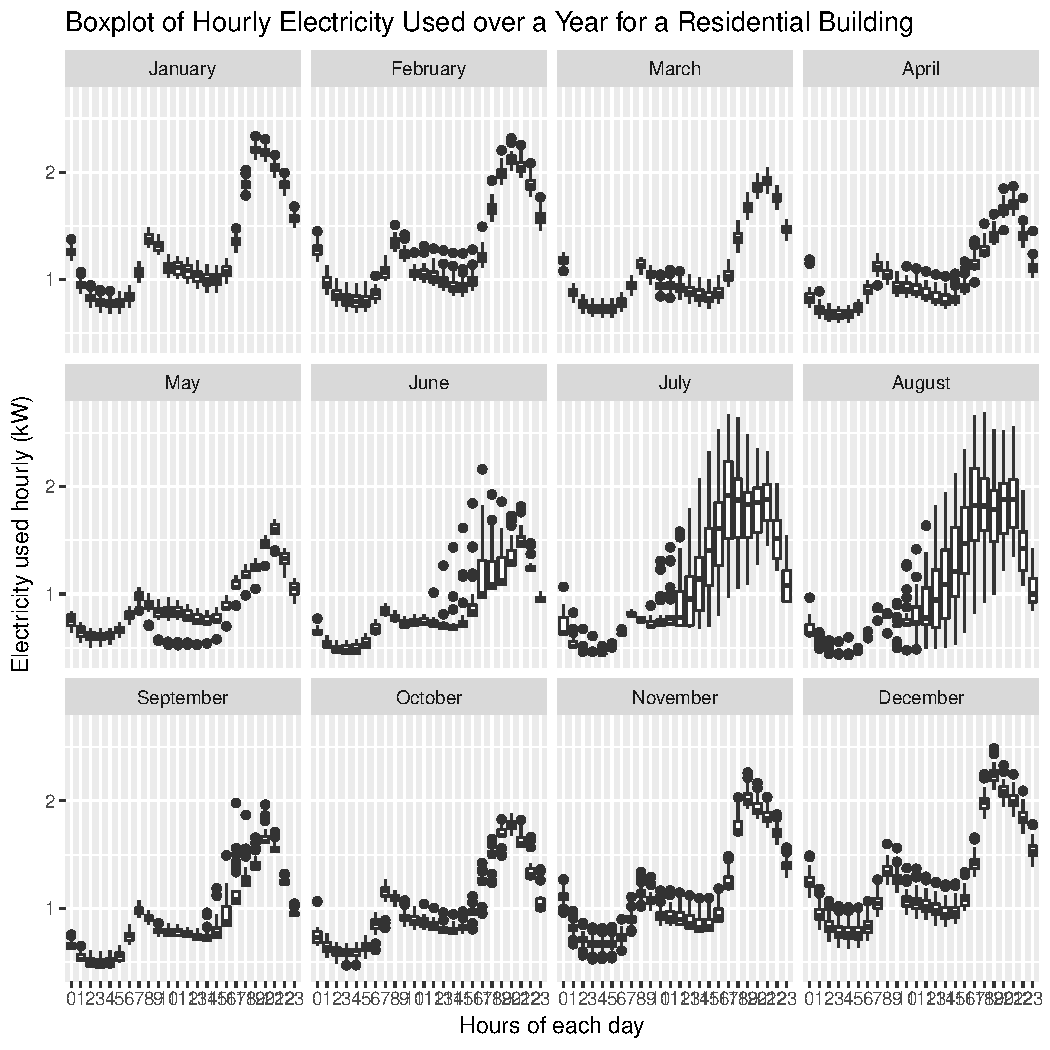
\includegraphics[width=\maxwidth]{figure/dirtyplots-1} 

\end{knitrout}

The plot shows that the residential building in question exhibits a similar pattern month on month throughout the year. There seems to be a smaller peak every day at 8am, and a larger peak later on at night at 9pm. \\

This is due to the natural cycle of a working day. Where a subject would wake up and use electricity in the morning for breakfast and showering before going to work, and the later peak explained by the person returning from work and requiring the use of lights, entertainment and cooking.\\

It can be seen that the total amount of electricity used per month differs. This can be explained by the relative temperature during each of the seasons. The winter months from December to February exhibit a higher overall average usage then other months, which can be explained by electrical heating. \\

The months of July and August exhibit a large variation of usage. This can be explained by the increase heat on certain days during the summer months.




\begin{knitrout}
\definecolor{shadecolor}{rgb}{0.969, 0.969, 0.969}\color{fgcolor}
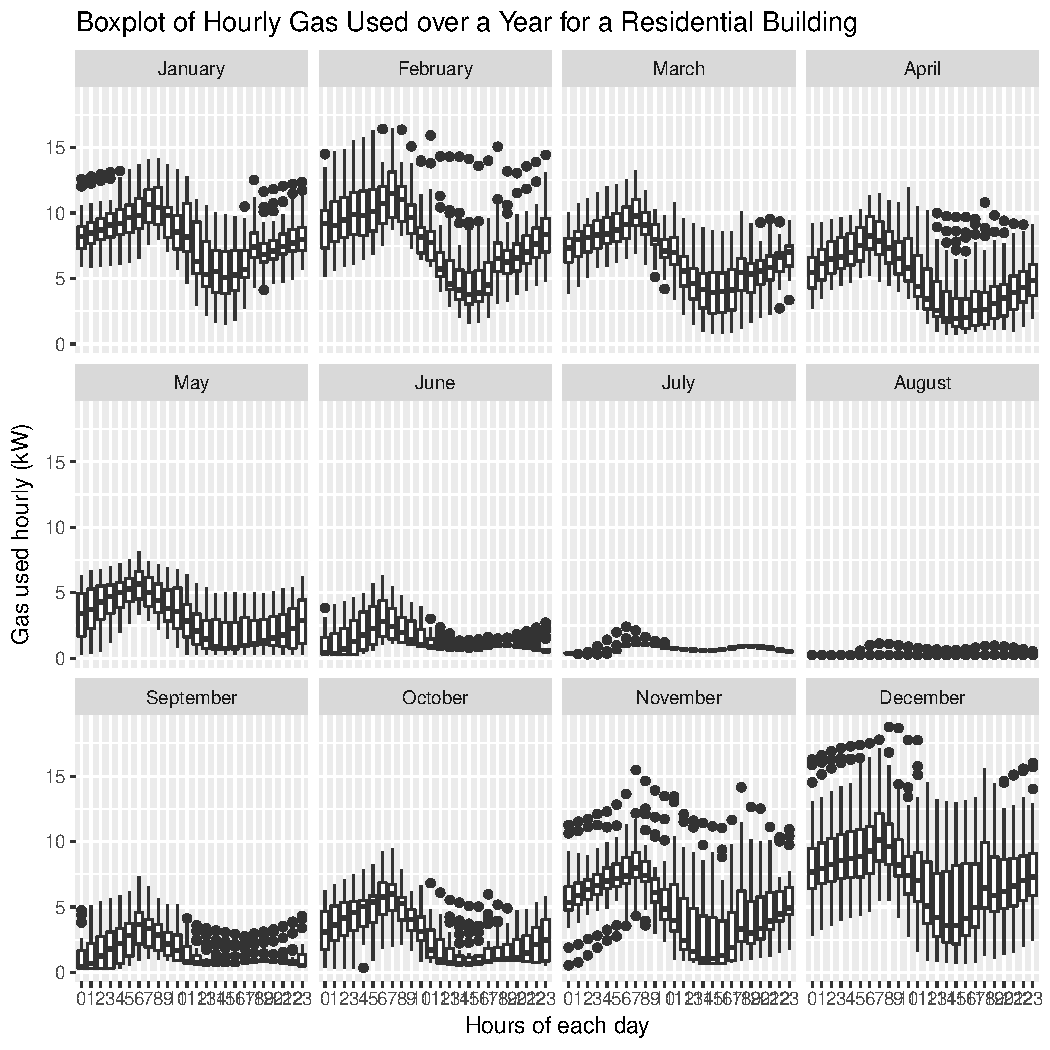
\includegraphics[width=\maxwidth]{figure/gas_plot-1} 

\end{knitrout}

The plot above shows the amount of gas used over a year for the same building in the previous plot. The difference in gas used between the summer and winter months is large here. With small amounts of gas used in July and August, and large amounts of gas used between November and February for heating purposes. \\

The plot below shows a subset of different building types. Here we see an electricity profile for different building types. 

\begin{knitrout}
\definecolor{shadecolor}{rgb}{0.969, 0.969, 0.969}\color{fgcolor}
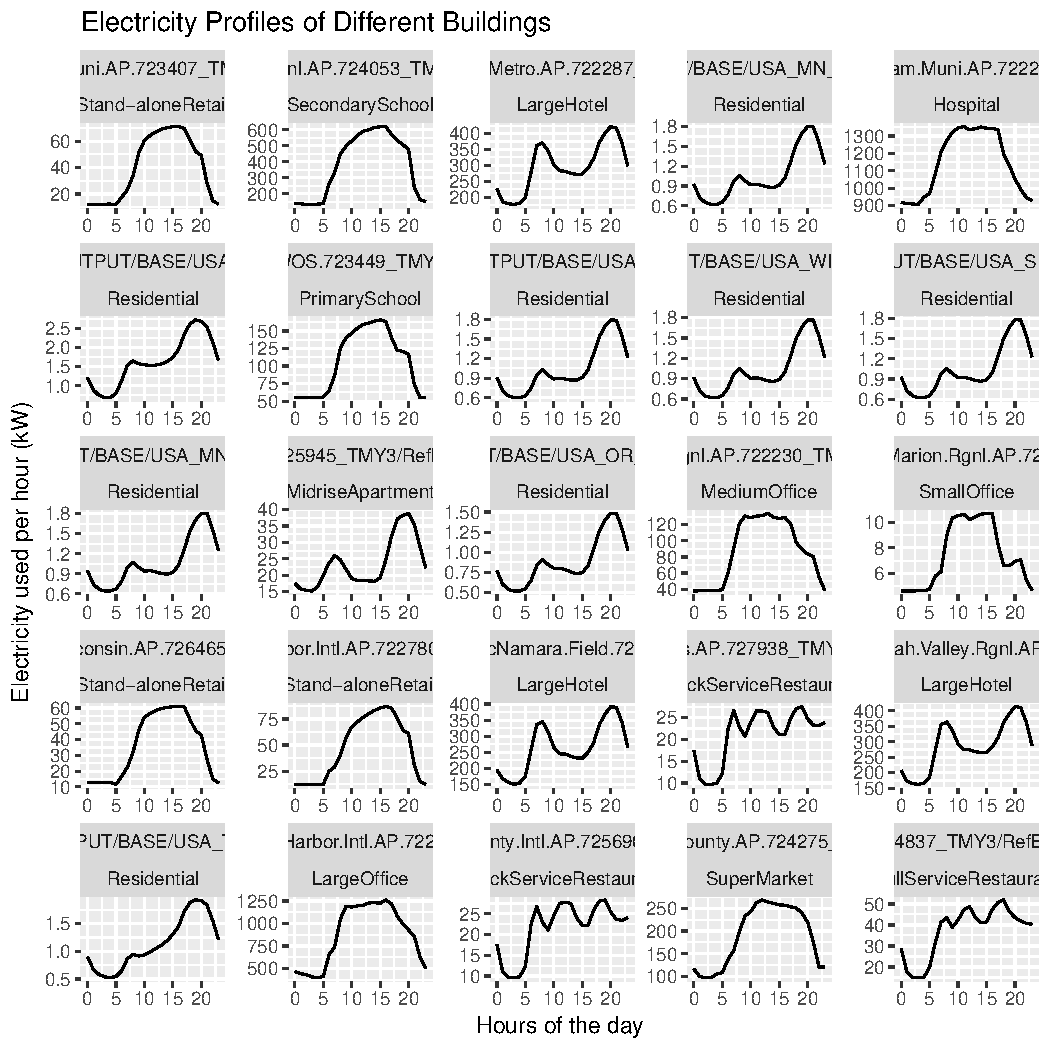
\includegraphics[width=\maxwidth]{figure/plot_different_profiles-1} 

\end{knitrout}

The electricity profiles can be split roughly into two categories. Residential properties and commercial properties.\\

Commercial properties have low energy usage outside of work hours, and high usage during work hours. This is opposite to that of residential properties which have peak times outside of the working day.\\

These characteristics are to be expected based on prior knowledge of human behaviour. \\

Apartments, residential properties, and hotels follow a similar pattern, whilst office, hospital, schools, and supermarkets follow another. Although offices, schools, and hospitals display similar patterns, they differ in total electricity usage.For instance, hospitals use a large amount of power. With a minimum amount of electricity of 900 kW, and a maximum of 1300kW at peak times. Secondary schools, however, use a minimum of 100 kW and maximum of 600kW. This can be explained by the relative requirements of each building, and overnight usage. \\

Restaurants follow a slightly different pattern where there are three peaks throughout the day. These peaks are during the hours of breakfast, lunch and dinner. The times that restaurants are busiest. \\


\subsection{Averaging of hourly data}

The data plotted was averaged to reduce the total length of the time series. The total length of the data per building was 8,760. Counting up the 15,000 CSV files, this makes up a huge amount of data. A lower diminesion would allow us to speed up the running of the algorithms, and at the same time preserve data. It can be seen from the plots above that a similar shape is recognised per day of the time series. This enables us to preserve the shape, and information of the time series. \\

A plot of the average hourly electricity used in a year, per hour is displayed below.

\begin{knitrout}
\definecolor{shadecolor}{rgb}{0.969, 0.969, 0.969}\color{fgcolor}\begin{kframe}


{\ttfamily\noindent\itshape\color{messagecolor}{\#\# Using avg\_elec\_p\_hour as value column: use value.var to override.}}\end{kframe}
\end{knitrout}

\begin{knitrout}
\definecolor{shadecolor}{rgb}{0.969, 0.969, 0.969}\color{fgcolor}
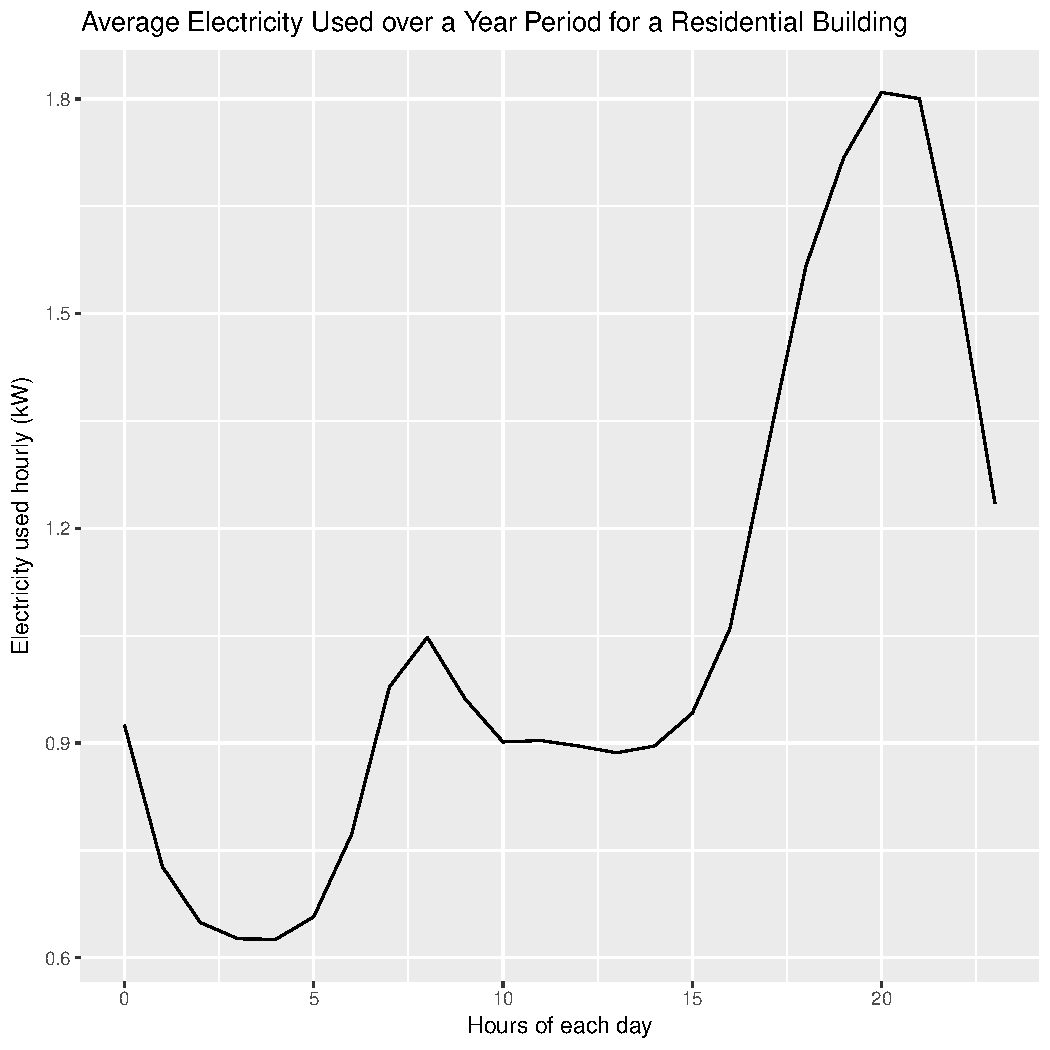
\includegraphics[width=\maxwidth]{figure/average-1} 

\end{knitrout}

The plot shows a shape consistent with the boxplots of the none averaged data over all months. It has also reduced the dimensionality of each time series by a factor of 365.\\

This data was used for classification in the subsequent 


\section{Clustering}

A lot of research has been undretaken for the classification of time series signals. Different methods are used such as feature extraction, similarity metrics of the raw data\cite{Wiens2009}, and model creation. \cite{WarrenLiao2005}

Here we used feature extraction, and similarity metrics to cluster the data. 



\subsection{Feature Extraction}

Feature extraction is a method to summarise the data using different metrics which explain the data.

The following table details the features extracted from the data. 
\begin{table}[]
\centering
\caption{My caption}
\label{my-label}
\begin{tabular}{ll}
\multicolumn{2}{c}{\textbf{Features Extracted}}                                                                 \\ \hline
\multicolumn{1}{|l|}{\textbf{Entire Time Series}}  & \multicolumn{1}{l|}{\textbf{Averaged Time Series by Hour}} \\ \hline
\multicolumn{1}{|l|}{Max Electricity Used}         & \multicolumn{1}{l|}{Number of peaks}                       \\ \hline
\multicolumn{1}{|l|}{Minimum Electricity Used}     & \multicolumn{1}{l|}{Highest Peak Time}                     \\ \hline
\multicolumn{1}{|l|}{Average Electricity Consumed} & \multicolumn{1}{l|}{Highest Peak Height}                   \\ \hline
\multicolumn{1}{|l|}{Total Number of Peaks}        & \multicolumn{1}{l|}{2nd Highest Peak Time}                 \\ \hline
\multicolumn{1}{|l|}{}                             & \multicolumn{1}{l|}{2nd Highest Peak Height}               \\ \hline
\multicolumn{1}{|l|}{}                             & \multicolumn{1}{l|}{Standard Deviation}                    \\ \hline
\multicolumn{1}{|l|}{}                             & \multicolumn{1}{l|}{Cumulative electricity used}           \\ \hline
\end{tabular}
\caption{Feature extraction for K Means Clustering}
\end{table}


Given these features we can map a time series to a vector of given features. These features allow us to compare different time series and enable us to cluster similar time series. 

\subsection{K-Clustering}

K Clustering is a technique which allows us to classify eliptical clusters of data using a predetermined number of clusters. It works based on an iterative approach of randomly initializing cluster centres, and moving each cluster, on each iteration, closer to the nearest cluster of data points.\\

Different plots were made to visualise the clustering of the K Clustering technique. A silhouette plot, a PCA plot, and a boxplot which displays the clusters in the time domain. These plots are explored below. 

A total of 12 clusters were chosen. This was done through visualisation using silhouette plots, and with the knowledge that there were 13 different buiding types. However, some of the building types can be put into the same category. For instance, full service restaurant and quick service restaurant.

A sample of 60 properties were taken to allow for plotting. 




A silhouette plot is a graphical display of how well points fit within a cluster. The silhouette shows which objects lie well within a cluster, and which ones are between clusters. Points with a score closer to 1 are well within their clusters, whereas points with a negative value, or value close to 0 could potentially fall in a different cluster.\\

By displaying all of the clusters in a single display it is possible to compare clusters, and can be used to select number of clusters. This is done by looking for a silhouette plot with the highest average silhouette widths, and looking for clusters containing a large amount of well positioned points. \cite{Rousseeuw1987}

\begin{knitrout}
\definecolor{shadecolor}{rgb}{0.969, 0.969, 0.969}\color{fgcolor}
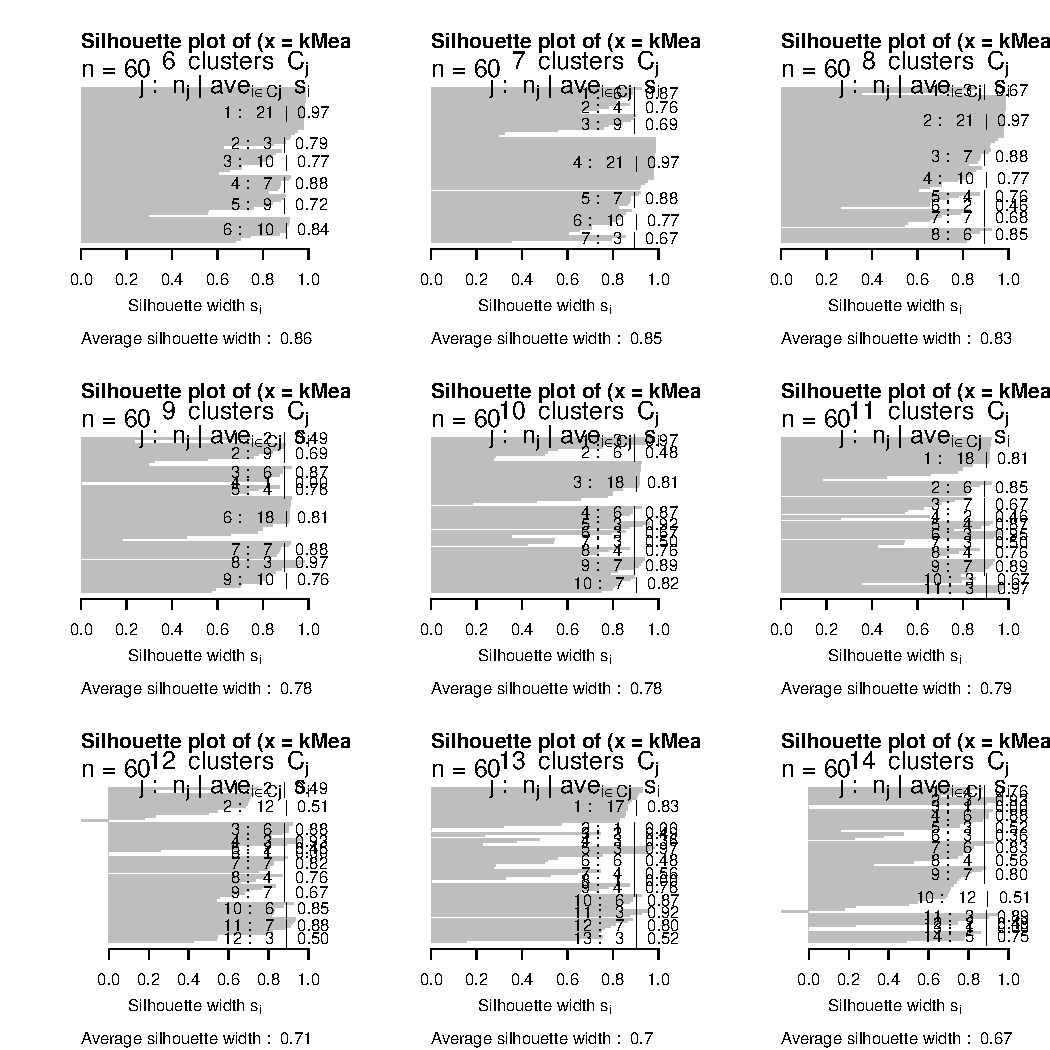
\includegraphics[width=\maxwidth]{figure/silhouette_k_plots-1} 

\end{knitrout}

Based on the silhouette plots, it would be most suitable to choose 6 or 8 numbers of clusters. This is because the silhouette width is higher the lower the number of clusters in this case. \\


The PCA plot enables us to plot many dimensions on two principal components. \\

The plot displays each of the features, and the points coloured by the cluster which they have been assigned to. 

The plot shows a wide spread of points, with natural clusters forming for particular types of buildings. Particularly restaurants, large hotels, small hotels, malls and retail, residential ,outpatients, and supermarkets.


However, upon further inspection, using a PCA plot it seems that judging solely by the silhouette width may not be enough. This is because there seems to be a large cluster towards the origin of the plot. As we move further away from the origin we seem to get clusters which are not bunched so close together. \\



\begin{knitrout}
\definecolor{shadecolor}{rgb}{0.969, 0.969, 0.969}\color{fgcolor}
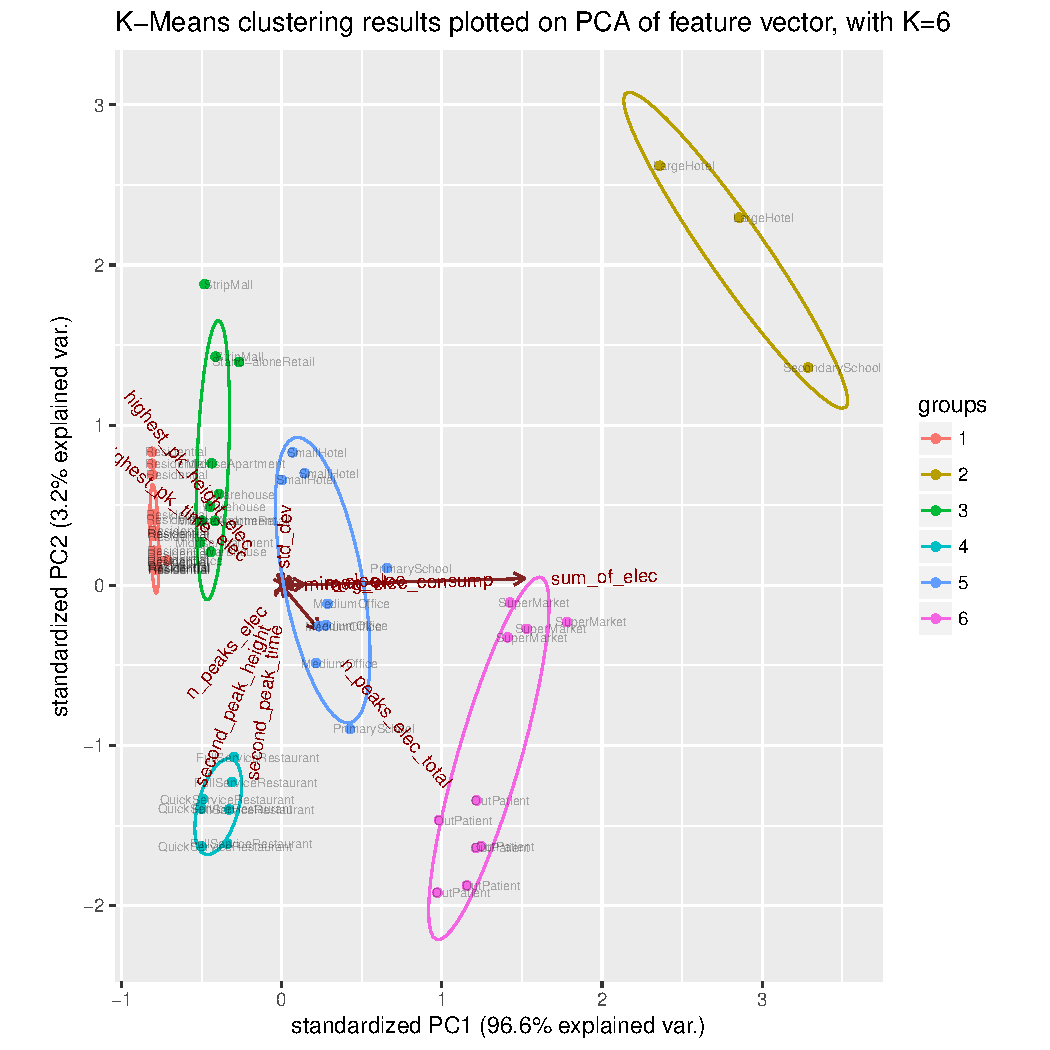
\includegraphics[width=\maxwidth]{figure/pca_plot-1} 

\end{knitrout}



\begin{knitrout}
\definecolor{shadecolor}{rgb}{0.969, 0.969, 0.969}\color{fgcolor}
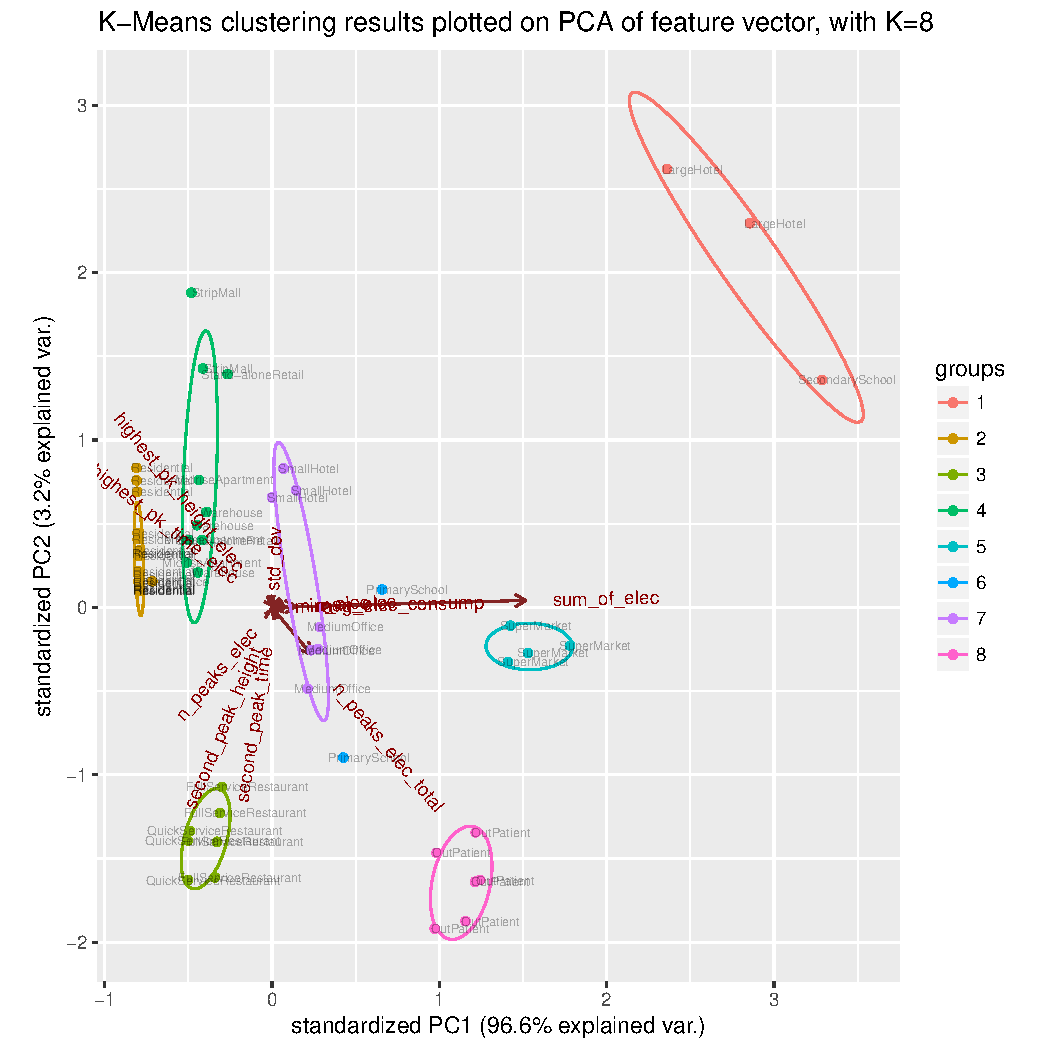
\includegraphics[width=\maxwidth]{figure/pca_plot_2-1} 

\end{knitrout}


It seems that a selection of k=8 seems to be optimal. This is because compared to 6, it correctly classifies supermarket and outpatient into their own categories, as well as creating a new category for primary school. \\

However, it does not create a seperate classification for warehouse and strip mall (cluster 4). To test this, we plotted the PCA result with K=9


\begin{knitrout}
\definecolor{shadecolor}{rgb}{0.969, 0.969, 0.969}\color{fgcolor}
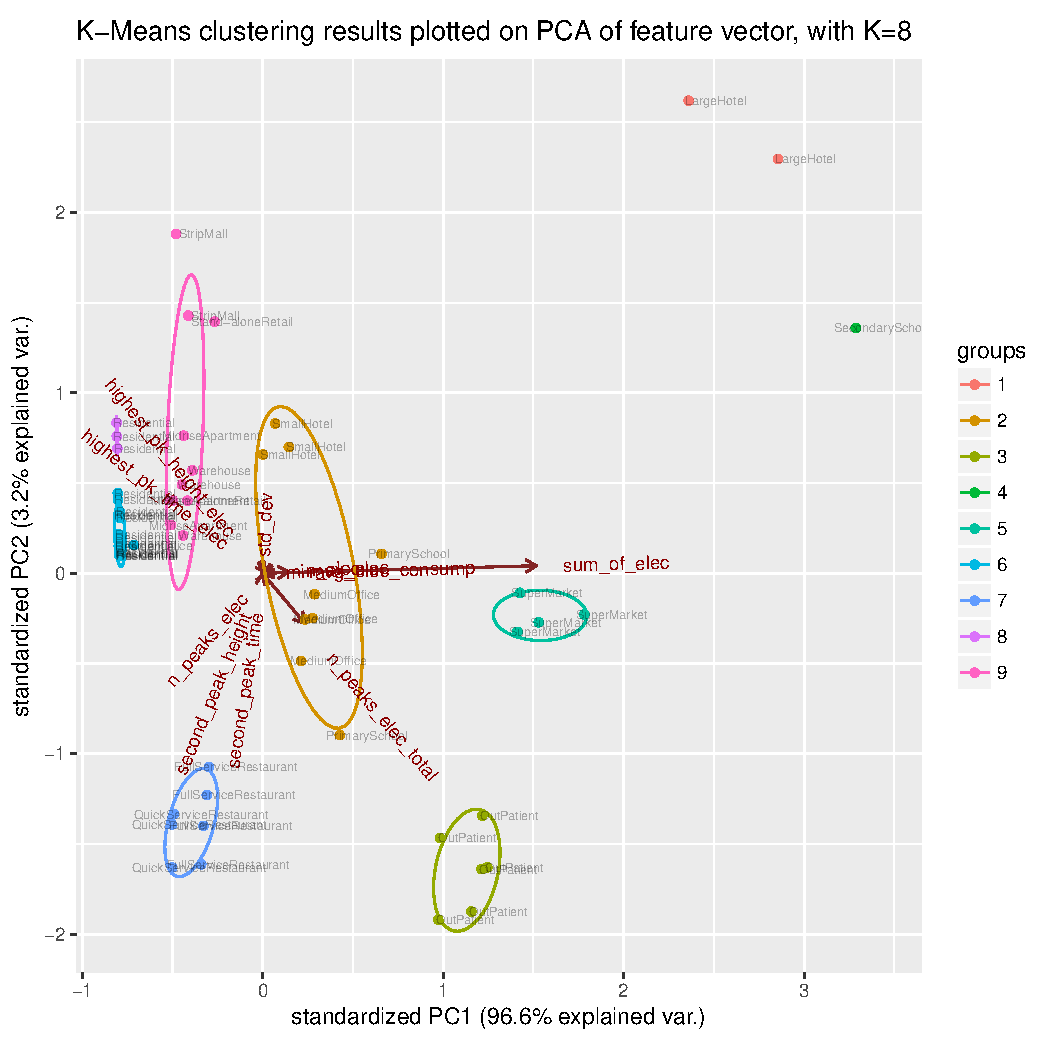
\includegraphics[width=\maxwidth]{figure/pca_plot_3-1} 

\end{knitrout}

Plotting a PCA of the results show that the additional group does not in fact create a seperate classificatoin for warehouse and strip mall, instead creating two classes for residential properties, which is incorrect. \\

I therefore left k=8.



We can also see properties which have not been clustered well, however the vast majority fit in clusters which are well assigned. 

\begin{knitrout}
\definecolor{shadecolor}{rgb}{0.969, 0.969, 0.969}\color{fgcolor}
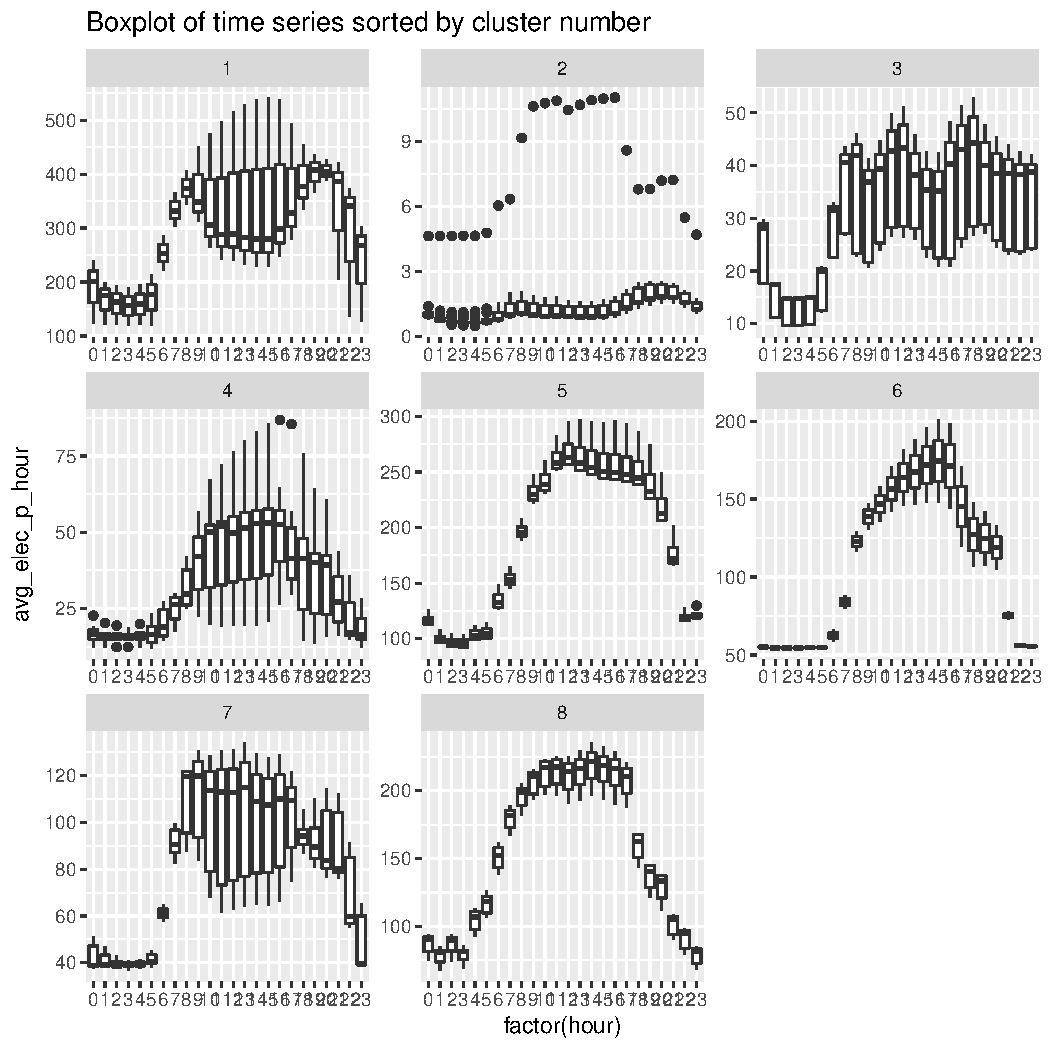
\includegraphics[width=\maxwidth]{figure/boxplot-1} 

\end{knitrout}

A plot of all of the data in boxplots shows distinct patterns of the buildings in the time domain. We can see, and compare the patterns to the original patterns, and the clusters of the PCA plot. Distinct patterns such as hotel, office, residential, outpatient, primary school, and restaurants can be seen. \\

There seems to be a single building which has been misclasified in plot number 2. This can be seen by the outlier plot, which seems to be a warehouse. However, it can be seen, which is ratified by the PCA plot, that the average time series is that of residential properties. 


\section{Hierarchical Clustering}

Hierarchical clustering is a clustering method which does not require a prespecified number of clusters. There are two strategies for hierarchical clustering, agglomerative or divisive.\\

Divisive starts by looking at the entire data, and initially splitting it into two clusters, and agglomerative starts with all of the data points and build up until there is one overall cluster. The clusters are split by forming different measures between clusters which I will not go into here.\\

Once a dendrogram is plotted groups can be seen based on the distance each group is from each other. \\

For the clustering we use the raw time series data, which is put through different dissimilarity metrics. These dissimilarity metrics calculate how different time series are from each other, based on measures such as euclidean distance. \\

Different dissimilarity metrics are described here.s

\subsection{Euclidean Distance}

Euclidean distance is a direct measure between points of different time series. Each point is compared to a point on a different time series, and the distance is calculated using the euclidean measure.

The output is shown below. A sample of 20 buildings were clustered for the purposes of visualisation.


\begin{knitrout}
\definecolor{shadecolor}{rgb}{0.969, 0.969, 0.969}\color{fgcolor}
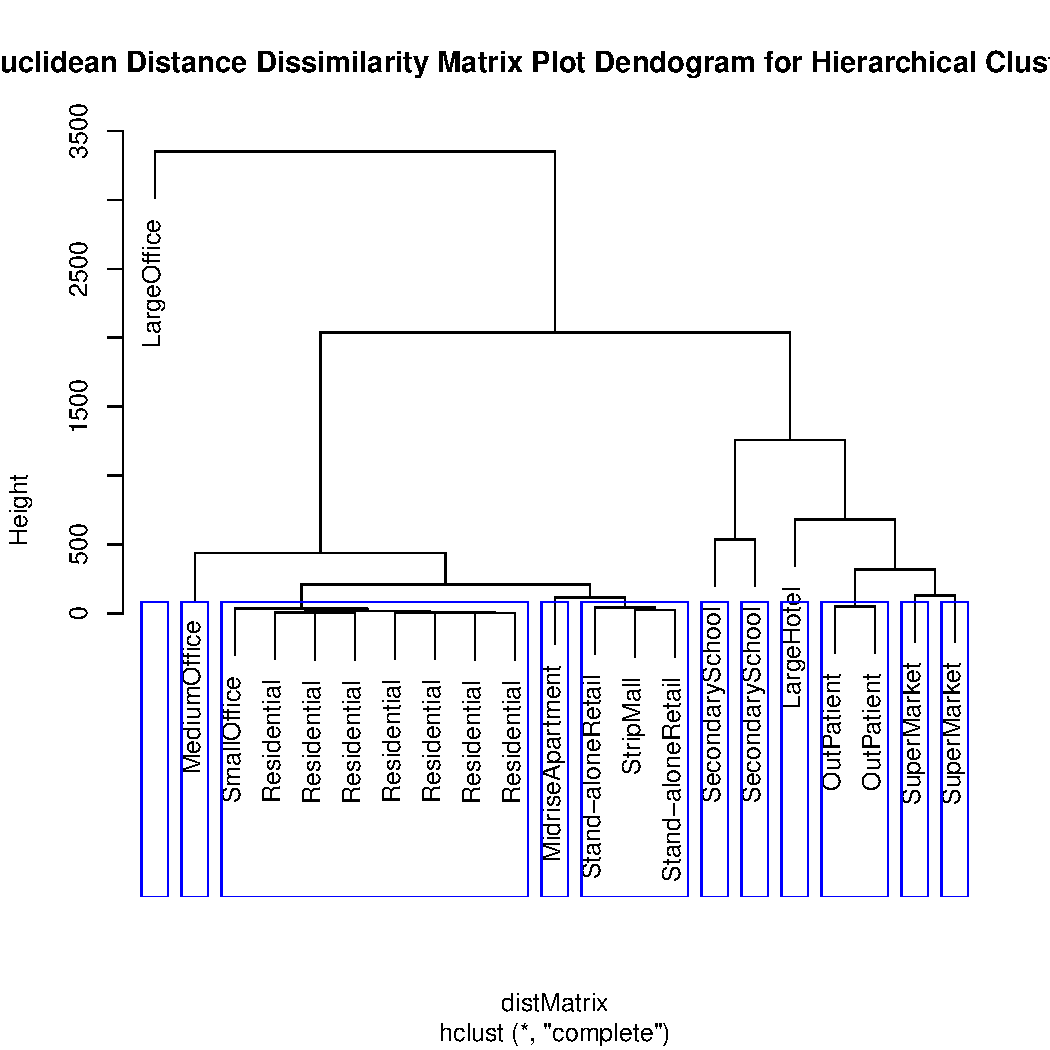
\includegraphics[width=\maxwidth]{figure/heirarchical_clustering-1} 

\end{knitrout}

The heirarchical clustering model performs well in correctly seperating the time series into closely related groups. For instance, all 7 of the residential properties fall within the same category. This is true also for supermarket, outpatient, and secondary school. \\

The accuracy of these clusters, visible in the dendogram plot seem to work better than the k-clustering technique which has more crossover.\\

The problem found, however, is the inability to explicity cut each of the clusters at a precise level. It can be seen that whilst the residential properties have been correctly classified into the same group, the two supermarkets, which are both in the same dendogram, are split into two levels. \\

There is a trade off at the cut off stage. Too high of a cut of a distance leads to too few groups, and too low leads to too many individual groups. Whilst a certain cut off distance works for a particular group, it may not work for another group.

\subsection{Dynamic Time Warping}

In this section we used dynamic time warping to calculate the dissimilarity matrix between different time series. \\

Dynamic time warping differs in the euclidean difference measure, in that it assumes that one time series is a time warped version of another. ie. The time series would be more similar if the time scale was scaled accordingly. Therefore, unlike the euclidean distance measure, each point is not strictly measured to the corresponding time on the other time series. 
\begin{knitrout}
\definecolor{shadecolor}{rgb}{0.969, 0.969, 0.969}\color{fgcolor}
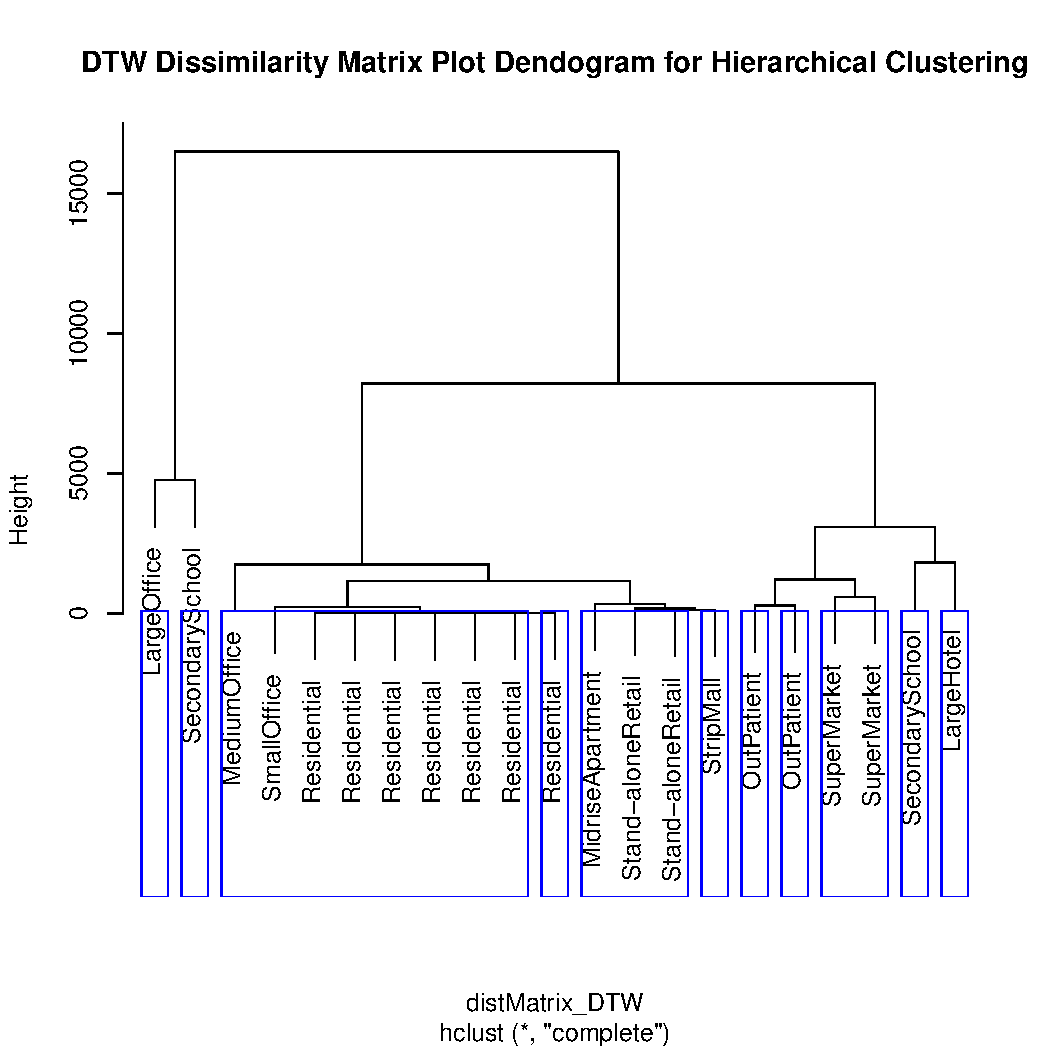
\includegraphics[width=\maxwidth]{figure/dynamic_time_warping-1} 

\end{knitrout}



\subsection{Wavelets}


Wavelets compute the frequency domain for a time series, based on subsets of time. We can therefore use the frequency information to compare time series for classification using a hierarchical clustering. \\

The euclidean distance between the wavelet approximations are calculated for use in the hierarchical model. 

\begin{knitrout}
\definecolor{shadecolor}{rgb}{0.969, 0.969, 0.969}\color{fgcolor}
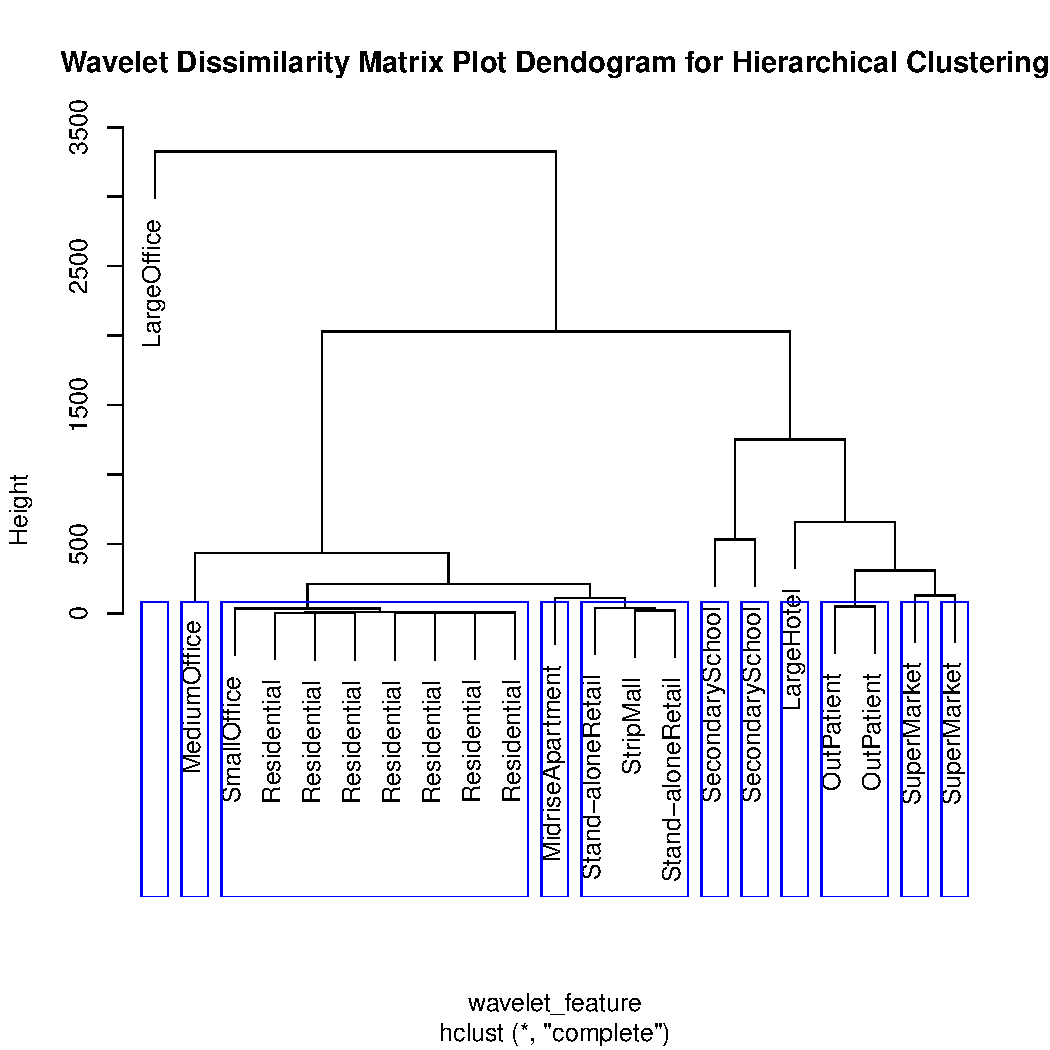
\includegraphics[width=\maxwidth]{figure/wavelet_diss-1} 

\end{knitrout}

The wavelet classification seems to work slightly better than that of dynamic time warping and euclidean distance. However a very similar structure exists, with slight in ordering.





\bibliographystyle{plain}
\bibliography{bibliography}


\end{document}
